\begin{table}[H]
\centering
\footnotesize
\definecolor{tabglobalgeneralotherunnorm0}{rgb}{0.7698,0.0196,0.1415}
\definecolor{tabglobalgeneralotherunnorm1}{rgb}{0.6671,0.0,0.149}
\definecolor{tabglobalgeneralotherunnorm2}{rgb}{0.7511,0.0068,0.1464}
\definecolor{tabglobalgeneralotherunnorm3}{rgb}{0.7558,0.01,0.1452}
\definecolor{tabglobalgeneralotherunnorm4}{rgb}{0.6596,0.0,0.149}
\definecolor{tabglobalgeneralotherunnorm5}{rgb}{0.7196,0.0,0.149}
\definecolor{tabglobalgeneralotherunnorm6}{rgb}{0.7418,0.0004,0.1489}
\definecolor{tabglobalgeneralotherunnorm7}{rgb}{0.6145,0.0,0.149}
\definecolor{tabglobalgeneralotherunnorm8}{rgb}{0.7346,0.0,0.149}
\definecolor{tabglobalgeneralotherunnorm9}{rgb}{0.502,0.0,0.149}
\definecolor{tabglobalgeneralotherunnorm10}{rgb}{0.5845,0.0,0.149}
\definecolor{tabglobalgeneralotherunnorm11}{rgb}{0.7271,0.0,0.149}
\definecolor{tabglobalgeneralotherunnorm12}{rgb}{0.5545,0.0,0.149}
\definecolor{tabglobalgeneralotherunnorm13}{rgb}{0.7464,0.0036,0.1476}
\definecolor{tabglobalgeneralotherunnorm14}{rgb}{0.532,0.0,0.149}
\definecolor{tabglobalgeneralotherunnorm15}{rgb}{0.6821,0.0,0.149}
\definecolor{tabglobalgeneralotherunnorm16}{rgb}{0.6446,0.0,0.149}
\definecolor{tabglobalgeneralotherunnorm17}{rgb}{1.0,0.9801,0.7513}
\definecolor{tabglobalgeneralotherunnorm18}{rgb}{1.0,0.9402,0.6538}
\definecolor{tabglobalgeneralotherunnorm19}{rgb}{0.9984,0.8971,0.5596}
\definecolor{tabglobalgeneralotherunnorm20}{rgb}{0.9961,0.8498,0.4615}
\definecolor{tabglobalgeneralotherunnorm21}{rgb}{0.9961,0.7634,0.3684}
\definecolor{tabglobalgeneralotherunnorm22}{rgb}{0.9955,0.6781,0.2894}
\definecolor{tabglobalgeneralotherunnorm23}{rgb}{0.9933,0.5962,0.254}
\definecolor{tabglobalgeneralotherunnorm24}{rgb}{0.991,0.4793,0.2143}
\definecolor{tabglobalgeneralotherunnorm25}{rgb}{0.9888,0.3398,0.1744}
\definecolor{tabglobalgeneralotherunnorm26}{rgb}{0.9463,0.2187,0.1412}
\definecolor{tabglobalgeneralotherunnorm27}{rgb}{0.8867,0.0996,0.1107}
\definecolor{tabglobalgeneralotherunnorm28}{rgb}{0.8025,0.042,0.1329}
\definecolor{tabglobalgeneralotherunnorm29}{rgb}{0.7046,0.0,0.149}
\definecolor{tabglobalgeneralotherunnorm30}{rgb}{0.5695,0.0,0.149}
\definecolor{tabglobalgeneralotherunnorm31}{rgb}{1.0,0.9779,0.7459}
\definecolor{tabglobalgeneralotherunnorm32}{rgb}{0.9991,0.9119,0.5906}
\definecolor{tabglobalgeneralotherunnorm33}{rgb}{0.9961,0.8066,0.4149}
\definecolor{tabglobalgeneralotherunnorm34}{rgb}{1.0,0.9756,0.7405}
\definecolor{tabglobalgeneralotherunnorm35}{rgb}{0.9961,0.7922,0.3994}
\definecolor{tabglobalgeneralotherunnorm36}{rgb}{1.0,0.9291,0.6268}
\definecolor{tabglobalgeneralotherunnorm37}{rgb}{0.9961,0.7058,0.3064}
\definecolor{tabglobalgeneralotherunnorm38}{rgb}{0.9944,0.6372,0.2717}
\definecolor{tabglobalgeneralotherunnorm39}{rgb}{0.9969,0.8676,0.4976}
\definecolor{tabglobalgeneralotherunnorm40}{rgb}{0.9894,0.3785,0.1855}
\definecolor{tabglobalgeneralotherunnorm41}{rgb}{0.9248,0.1739,0.1292}
\definecolor{tabglobalgeneralotherunnorm42}{rgb}{0.9963,0.8553,0.4718}
\definecolor{tabglobalgeneralotherunnorm43}{rgb}{0.9709,0.2699,0.155}
\definecolor{tabglobalgeneralotherunnorm44}{rgb}{0.9974,0.8774,0.5183}
\definecolor{tabglobalgeneralotherunnorm45}{rgb}{0.9887,0.332,0.1722}
\definecolor{tabglobalgeneralotherunnorm46}{rgb}{0.9217,0.1675,0.1275}
\definecolor{tabglobalgeneralotherunnorm47}{rgb}{0.577,0.0,0.149}
\begin{minipage}{0.34\textwidth}
\centering
\footnotesize vs.\ topological\\[3pt]
\renewcommand{\arraystretch}{1.2}
\begin{tabular}{lccc}
\toprule
Checkpoint & First & Middle & Last \\
\midrule
0 & \cellcolor{tabglobalgeneralotherunnorm0}\textcolor{white}{$0.437 \pm 0.041$} & \cellcolor{tabglobalgeneralotherunnorm1}\textcolor{white}{$0.468 \pm 0.049$} & \cellcolor{tabglobalgeneralotherunnorm2}\textcolor{white}{$0.446 \pm 0.042$} \\
1 & \cellcolor{tabglobalgeneralotherunnorm3}\textcolor{white}{$0.443 \pm 0.039$} & \cellcolor{tabglobalgeneralotherunnorm4}\textcolor{white}{$0.472 \pm 0.048$} & \cellcolor{tabglobalgeneralotherunnorm5}\textcolor{white}{$0.455 \pm 0.039$} \\
5 & \cellcolor{tabglobalgeneralotherunnorm6}\textcolor{white}{$0.449 \pm 0.037$} & \cellcolor{tabglobalgeneralotherunnorm7}\textcolor{white}{$0.483 \pm 0.043$} & \cellcolor{tabglobalgeneralotherunnorm1}\textcolor{white}{$0.469 \pm 0.034$} \\
15 & \cellcolor{tabglobalgeneralotherunnorm8}\textcolor{white}{$0.451 \pm 0.038$} & \cellcolor{tabglobalgeneralotherunnorm9}\textcolor{white}{$0.515 \pm 0.043$} & \cellcolor{tabglobalgeneralotherunnorm10}\textcolor{white}{$0.491 \pm 0.038$} \\
50 & \cellcolor{tabglobalgeneralotherunnorm11}\textcolor{white}{$0.452 \pm 0.038$} & \cellcolor{tabglobalgeneralotherunnorm12}\textcolor{white}{$0.500 \pm 0.042$} & \cellcolor{tabglobalgeneralotherunnorm1}\textcolor{white}{$0.470 \pm 0.040$} \\
200 & \cellcolor{tabglobalgeneralotherunnorm13}\textcolor{white}{$0.447 \pm 0.034$} & \cellcolor{tabglobalgeneralotherunnorm14}\textcolor{white}{$0.506 \pm 0.042$} & \cellcolor{tabglobalgeneralotherunnorm15}\textcolor{white}{$0.466 \pm 0.042$} \\
last & \cellcolor{tabglobalgeneralotherunnorm8}\textcolor{white}{$0.451 \pm 0.035$} & \cellcolor{tabglobalgeneralotherunnorm14}\textcolor{white}{$0.505 \pm 0.042$} & \cellcolor{tabglobalgeneralotherunnorm16}\textcolor{white}{$0.476 \pm 0.043$} \\
\bottomrule
\end{tabular}
\end{minipage}%
\hfill
\begin{minipage}{0.085\textwidth}
\centering
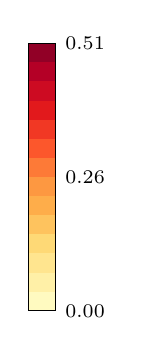
\begin{tikzpicture}
\fill[tabglobalgeneralotherunnorm17] (0,0.0000) rectangle (0.35,0.2429);
\fill[tabglobalgeneralotherunnorm18] (0,0.2429) rectangle (0.35,0.4857);
\fill[tabglobalgeneralotherunnorm19] (0,0.4857) rectangle (0.35,0.7286);
\fill[tabglobalgeneralotherunnorm20] (0,0.7286) rectangle (0.35,0.9714);
\fill[tabglobalgeneralotherunnorm21] (0,0.9714) rectangle (0.35,1.2143);
\fill[tabglobalgeneralotherunnorm22] (0,1.2143) rectangle (0.35,1.4571);
\fill[tabglobalgeneralotherunnorm23] (0,1.4571) rectangle (0.35,1.7000);
\fill[tabglobalgeneralotherunnorm24] (0,1.7000) rectangle (0.35,1.9429);
\fill[tabglobalgeneralotherunnorm25] (0,1.9429) rectangle (0.35,2.1857);
\fill[tabglobalgeneralotherunnorm26] (0,2.1857) rectangle (0.35,2.4286);
\fill[tabglobalgeneralotherunnorm27] (0,2.4286) rectangle (0.35,2.6714);
\fill[tabglobalgeneralotherunnorm28] (0,2.6714) rectangle (0.35,2.9143);
\fill[tabglobalgeneralotherunnorm29] (0,2.9143) rectangle (0.35,3.1571);
\fill[tabglobalgeneralotherunnorm30] (0,3.1571) rectangle (0.35,3.4000);
\draw[black,line width=0.3pt] (0,0) rectangle (0.35,3.4000);
\node[right,font=\scriptsize,anchor=west] at (0.35,3.4000) {0.51};
\node[right,font=\scriptsize,anchor=west] at (0.35,1.7000) {0.26};
\node[right,font=\scriptsize,anchor=west] at (0.35,0) {0.00};
\end{tikzpicture}
\end{minipage}%
\hfill
\begin{minipage}{0.34\textwidth}
\centering
\footnotesize vs.\ zero\\[3pt]
\renewcommand{\arraystretch}{1.2}
\begin{tabular}{lccc}
\toprule
Checkpoint & First & Middle & Last \\
\midrule
0 & \cellcolor{tabglobalgeneralotherunnorm31}\textcolor{black}{$0.172 \pm 0.143$} & \cellcolor{tabglobalgeneralotherunnorm32}\textcolor{black}{$0.650 \pm 0.597$} & \cellcolor{tabglobalgeneralotherunnorm33}\textcolor{black}{$1.203 \pm 1.128$} \\
1 & \cellcolor{tabglobalgeneralotherunnorm34}\textcolor{black}{$0.188 \pm 0.145$} & \cellcolor{tabglobalgeneralotherunnorm19}\textcolor{black}{$0.735 \pm 0.648$} & \cellcolor{tabglobalgeneralotherunnorm35}\textcolor{black}{$1.249 \pm 1.128$} \\
5 & \cellcolor{tabglobalgeneralotherunnorm36}\textcolor{black}{$0.530 \pm 0.331$} & \cellcolor{tabglobalgeneralotherunnorm37}\textcolor{black}{$1.537 \pm 0.908$} & \cellcolor{tabglobalgeneralotherunnorm38}\textcolor{black}{$1.785 \pm 1.072$} \\
15 & \cellcolor{tabglobalgeneralotherunnorm39}\textcolor{black}{$0.933 \pm 0.540$} & \cellcolor{tabglobalgeneralotherunnorm40}\textcolor{black}{$2.458 \pm 1.259$} & \cellcolor{tabglobalgeneralotherunnorm41}\textcolor{white}{$2.943 \pm 1.615$} \\
50 & \cellcolor{tabglobalgeneralotherunnorm42}\textcolor{black}{$1.027 \pm 0.658$} & \cellcolor{tabglobalgeneralotherunnorm43}\textcolor{white}{$2.697 \pm 1.388$} & \cellcolor{tabglobalgeneralotherunnorm7}\textcolor{white}{$3.922 \pm 1.849$} \\
200 & \cellcolor{tabglobalgeneralotherunnorm44}\textcolor{black}{$0.875 \pm 0.672$} & \cellcolor{tabglobalgeneralotherunnorm45}\textcolor{white}{$2.548 \pm 1.593$} & \cellcolor{tabglobalgeneralotherunnorm9}\textcolor{white}{$4.179 \pm 2.132$} \\
last & \cellcolor{tabglobalgeneralotherunnorm39}\textcolor{black}{$0.938 \pm 0.705$} & \cellcolor{tabglobalgeneralotherunnorm46}\textcolor{white}{$2.968 \pm 1.895$} & \cellcolor{tabglobalgeneralotherunnorm47}\textcolor{white}{$4.006 \pm 1.898$} \\
\bottomrule
\end{tabular}
\end{minipage}%
\hfill
\begin{minipage}{0.085\textwidth}
\centering
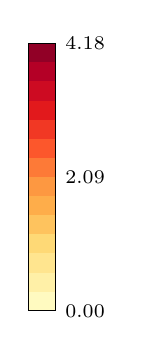
\begin{tikzpicture}
\fill[tabglobalgeneralotherunnorm17] (0,0.0000) rectangle (0.35,0.2429);
\fill[tabglobalgeneralotherunnorm18] (0,0.2429) rectangle (0.35,0.4857);
\fill[tabglobalgeneralotherunnorm19] (0,0.4857) rectangle (0.35,0.7286);
\fill[tabglobalgeneralotherunnorm20] (0,0.7286) rectangle (0.35,0.9714);
\fill[tabglobalgeneralotherunnorm21] (0,0.9714) rectangle (0.35,1.2143);
\fill[tabglobalgeneralotherunnorm22] (0,1.2143) rectangle (0.35,1.4571);
\fill[tabglobalgeneralotherunnorm23] (0,1.4571) rectangle (0.35,1.7000);
\fill[tabglobalgeneralotherunnorm24] (0,1.7000) rectangle (0.35,1.9429);
\fill[tabglobalgeneralotherunnorm25] (0,1.9429) rectangle (0.35,2.1857);
\fill[tabglobalgeneralotherunnorm26] (0,2.1857) rectangle (0.35,2.4286);
\fill[tabglobalgeneralotherunnorm27] (0,2.4286) rectangle (0.35,2.6714);
\fill[tabglobalgeneralotherunnorm28] (0,2.6714) rectangle (0.35,2.9143);
\fill[tabglobalgeneralotherunnorm29] (0,2.9143) rectangle (0.35,3.1571);
\fill[tabglobalgeneralotherunnorm30] (0,3.1571) rectangle (0.35,3.4000);
\draw[black,line width=0.3pt] (0,0) rectangle (0.35,3.4000);
\node[right,font=\scriptsize,anchor=west] at (0.35,3.4000) {4.18};
\node[right,font=\scriptsize,anchor=west] at (0.35,1.7000) {2.09};
\node[right,font=\scriptsize,anchor=west] at (0.35,0) {0.00};
\end{tikzpicture}
\end{minipage}
\caption{Global Wasserstein alignment, GeneralSheaf other Laplacian: maps trained \texttt{norm=True}, evaluated unnormalised. Mean $\pm$ SE across 10 datasets (First/Last), 8 for Middle (datasets with $L=2$ contribute no middle layer). Cell shading (each block independently scaled): white = 0, dark red = block maximum, YlOrRd colormap.}
\label{tab:global_general_other_unnorm}
\end{table}
